\documentclass[Softwaredesign/Softwaredesign_main.tex]{subfiles}
\begin{document}

\section{CupSensor\_IF}
Der skal udvikles en CupSensor\_IF klasse på PlayerSideApp som har til opgave at håndtere input/output for alle 6 Cup Sensors på en player side. Dette er udvilket på baggrund af hardwaren beskrevet i \ref{hwdesign:sec:CupSensor}. Som opsummering benyttes der en multiplexer som styre hvilken cup sensor som der sættes til blinke med dens IR LED. Herefter bruges der udtrykket der styres hvilke 'sensor der læses'. Multiplexeren styres af et register Control\_Reg\_Led. Inputtet ender med at blive læst med en Delta Sigma ADC, med et differentiabelt input. Til forventede signaler er der kun positive signaler. Der benyttes sinc4 filteret i ADC'en. Dette betyder at udgangen først er korrekt efter 4 samples hvis der sker et step i indgangssignalet. Til at læse signalet fra ADC'en benyttes en DMA (Direct memory access) komponent som genererer et interrupt når den er færdig.

Der er til software design af CupLight\_IF, udviklet et klassediagram. Diagrammet kan ses på figur \ref{fig:CupSensor-IF-classDiagram}. Det vil være uhensigtsmæssigt at lave alt i en klasse. Klassen CupSensor\_IF er den klasse som GameController interagere med. De resterende klasser er en del af en custom component i PSoC\autocite{PSoCHowToCreateCustomComponents}. CupSensor er hoved-klassen for CupSensor blokken. Den skal som alle andre PSoC komponenter startes vha. Start metoden. Denne metode sørge for at starte og opsætte de forskellige hardware komponenter og interrupts. Derudover skal de 6 instanser for CupSensorUnit initieres. Som en del af denne metode skal DMA'en opsættes. Koden til dette genereres vha. PSoC Creators DMA Wizard\autocite[2]{DMADatasheet}. Da man som tidligere beskrevet skal vente 4 samples efter et step på indgangen, opsættes DMA'en til kun at generere et interrupt efter hver 6. sample. Det er 6 frem for 4 Da andre dele af systemet også vil tage noget tid at reagere på et step. Det step der tales om, er ændringen i hvilken sensor der sættes til at blinke. Da to sensorer ikke nødvendigvis har samme output, vil ændringen opfattes som et step. ADC'en har en samplerate på 2500 sps, når kun hver 6. måling er brugbar svare det til en samplerate på ca. 417 sps. Men da der skal læses fra 6 Cup Sensors, er sampleraten for en given sensor kun ca 70 sps. Dette vil betyde at at den maksimale frekvens der kan måles er 35Hz, eller signaler med en periode på ca 29 ms eller længere. Det signal der for sensoren skal analyseres som har den højeste frekvens er når en bold rammer i. Dette har en periode på ca 200ms. Derfor er dette en god nok løsning.

Der skal i CupSensor klassen være get metoderne til CupStatus og HitStatus. Det er metoderne getStatus() og getHitStatus(). Der er det to funktioner statusCallback og hitStatusCallback som har funktionspointere som argumenter. Disse funktioner bruges til at indstille hvilken metode der skal kaldes når cupStatus eller hitStatus ændres. Disse metoder kaldes af CupSensor\_IF klassen som sørger for at de to funktioner der kaldes er updateCupStatus og updateHitStatus i GameController klassen (i PlayerSideApp).
Som tidligere beskrevet sker der et interrupt når der er en ny måling fra ADC'en (kun hver 6. måling). Til dette interrupt er der en ISR kaldes CY\_ISR(newValueInterruptHandler). Indholdet af denne interrupt handler kan ses på figur \ref{fig:CupSensor-IF-getting-reading}. 
 
\begin{figure}[H]
    \centering
    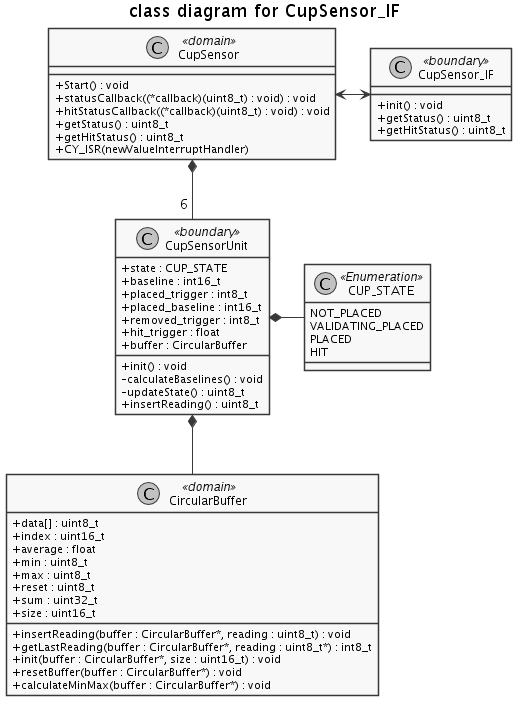
\includegraphics[width=0.8\textwidth]{Softwaredesign/CupSensor_IF/graphics/classDiagram.png}
    \caption{.}
    \label{fig:CupSensor-IF-classDiagram}
\end{figure}

Der er 6 objekter af klassen CupSensorUnit. Denne repræsentere hver Cup Sensor. Hver CupSensorUnit har en CUP\_STATE til at holde styr på tilstanden af den givne Cup Sensor. Derudover er der en CircularBuffer klasse som bruges til at lagre de seneste målinger for hver CupSensorUnit.

Til at styre tilstanden for CupSensorUnit udvikles en tilstandsmaskine som ses på figur \ref{fig:CupSensor-IF-state}. Der er af åbenlyse grunde de tre tilstande NOT\_PLACE, PLACED og HIT. Men der er også en tilstand VALIDATING\_PLACED. Denne tilstand er til for at minimere risikoen for at der sker en falsk transition til tilstanden PLACED, da det kræver at signalet skal være højt i en længere tid, 20 samples eller ca. 300ms. Dette vil gøre systemet langsommere, men mere pålideligt. Som det ses på figur \ref{fig:CupSensor-IF-state}, benyttes der 'baseline'. Dette er inspiration fra CapSense, som blev undersøgt i teknologiundersøgelsen. CapSense benytter et lavpas filter som beregner et baseline som trækkes fra alle de rå målinger. Der er valgt at benytte noget lignende. Hvor der er to 'baselines'. \textbf{baseline} og \textbf{placed\_baseline}. \textbf{baseline} er gennemsnitsværdien for når der ikke er placeret en kop. Dette er for at kunne detektere at en kop bliver placeret, da der kan være forskellige omstændigheder der gør at baseline vil ændre sig. Så det muligvis ikke vil være muligt at benytte absolutte værdier der bestemmer hvornår der er en kop. For at detektere at en bold rammer i benyttes der \textbf{placed\_baseline}, som bruges til at detektere at en bold rammer i. Dette er brugt da der ikke nødvendigvis er det samme signal med forskellige mængder øl. \textbf{placed\_baseline} er relativ til \textbf{baseline}. Det der benævnes 'reading', er den målte værdi minus den beregnede \textbf{baseline}. Til at skifte mellem de forskellige tilstande benyttes der forskellige grænseværdier som reading skal være over/under. Til at skifte til tilstanden VALIDATING\_PLACED og tilbage til NOT\_PLACED, både fra VALIDATING\_PLACED, PLACED og HIT, benyttes der absolutte grænseværdier, placed\_trigger og removed\_trigger. Men til at skifte til HIT benyttes der en grænseværdi, hit\_trigger, der er relativ til værdien, placed\_baseline, når der er placeret en kop. Dette er til for at der fx. for en kop med meget øl, og derfor lille placed\_baseline, skal en mindre absolut ændring til for at detektere at en bold rammer i. Der vil komme en mindre ændring da bolden vil være længere væk fra sensoren.
\begin{figure}[H]
    \centering
    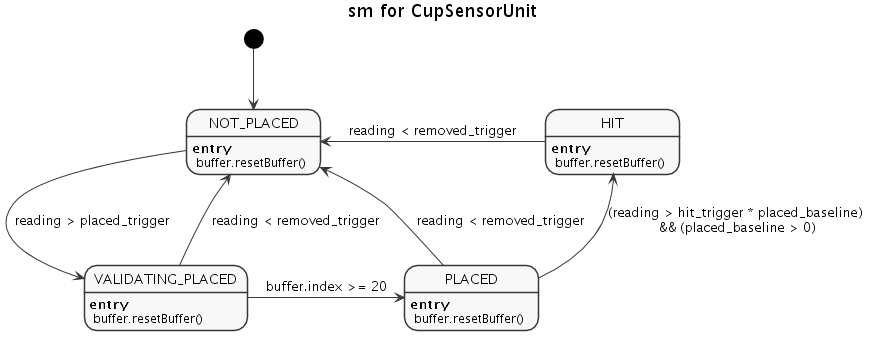
\includegraphics[width=1\textwidth]{Softwaredesign/CupSensor_IF/graphics/state.png}
    \caption{.}
    \label{fig:CupSensor-IF-state}
\end{figure}

Der kan ses på sekvensdiagrammet på figur \ref{fig:CupSensor-IF-getting-reading} hvad der sker når der modtages en ny måling fra ADC'en. Det første der sker er at ændre på hvilken sensor der læses. Dette gøres ved at ændre på Control\_Reg\_Led registeret. Denne komponent har sin egen 'klasse' hvor Read funktionen bruges til at læse hvad den nuværende tilstand værdi er. Herefter opdateres dens værdi ved at tælle én op. Der sørges desuden for at Control\_Reg\_Led kun vil nå op til 5, hvorefter den skifter til 0. 
Efter dette kaldes insertReading metoden i den CupSensorUnit som læsningen stammer fra, bestemt af værdien af Control\_Reg\_Led. Denne metode indsætter værdien i dens buffer, som er en CicularBuffer. Herefter kaldes updateState som på baggrund af den nye værdi og de beregnede 'baselines', opdatere tilstanden i tilstandsmaskinen. \textbf{buffer} bruges hovedsagligt til at beregne et gennemsnit, da det skal bruges til at beregne 'baselines' som skal beregnes når calculateBaselines kaldes. Denne funktion beregner ud fra gennemsnittet af bufferen de to 'baselines' \textbf{baseline} og \textbf{placed\_baseline}. calculateBaselines beregner og opdatere \textbf{baseline} hvis tilstanden er NOT\_PLACED. Hvis tilstanden er PLACED beregnes og opdateres \textbf{placed\_baseline}.
insertReading metoden i CupSensor klassen returnerer om tilstanden ændres. Hvis tilstanden ændres opdateres den nødvendige bit i cupStatus og hitStatus, bestemt af værdien af Control\_Reg\_Led. bit'et i cupStatus ændres til 1 når tilstanden skifter til PLACED og til 0 når tilstanden skifter til NOT\_PLACED. bit'et i hitStatus skifter til 1 når tilstanden skifter til HIT og til 0 når tilstanden skifter til NOT\_PLACED. 
\begin{figure}[H]
    \centering
    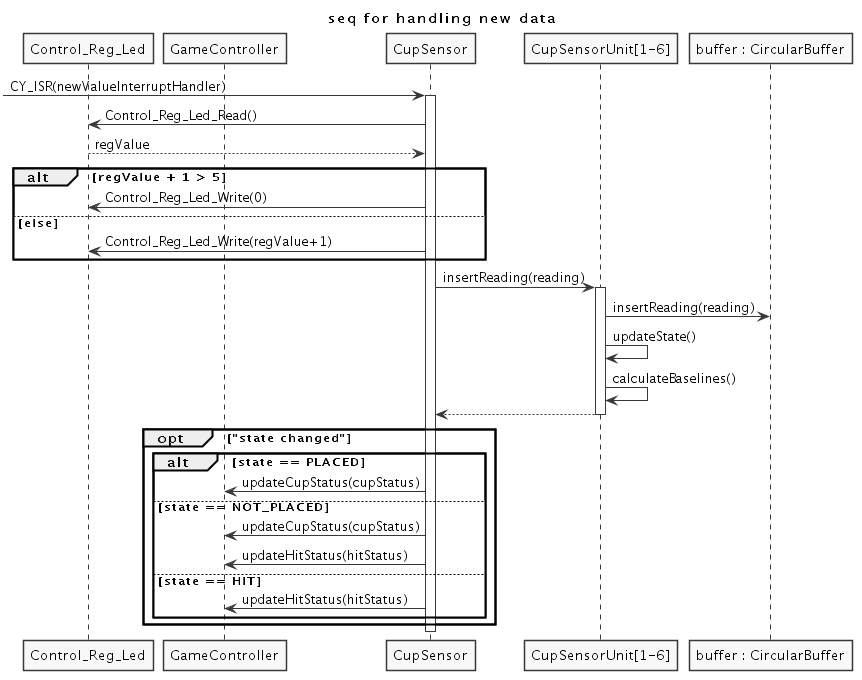
\includegraphics[width=1\textwidth]{Softwaredesign/CupSensor_IF/graphics/getting_reading.png}
    \caption{.}
    \label{fig:CupSensor-IF-getting-reading}
\end{figure}

\subsection{Valg af grænseværdier} \label{sec:CupSensorThresholds}
Til at bestemme de forskellige grænseværdier er der udført nogle målinger, hvor der placeres/fjernes en kop flere gange, og der tabes en bold flere gange. Dette udføres med forskellige mængder øl, den øvre (130ml) og nedre (90ml) grænse for mængden af øl beskrevet i kravene samt den nominiele værdi, 110ml. Disse målinger laves hvor den læste værdi skrives til en DAC med en opløsning på 16mV. De læste målinger divideres med 16mV for at opnå talværdien som systemet bruger. Der afrundes til nærmeste heltal. Målingerne udføres med Digilent Analog Discovery 2\autocite{AnalogDiscovery2}.

Først laves der målinger der måler baseline for den givne opstilling

\begin{table}[H]
    \centering
    \begin{tabular}{|L{0.2\textwidth}|L{0.15\textwidth}|}
        \hline
        \textbf{Måling nr.} & \textbf{værdi} \\ \hline
        1 & 30 \\ \hline
        2 & 29 \\ \hline
        3 & 29 \\ \hline
        4 & 29 \\ \hline
        5 & 29 \\ \hline
        6 & 29 \\ \hline
        7 & 29 \\ \hline
        8 & 29 \\ \hline
        9 & 29 \\ \hline
        10 & 29 \\ \hline
    \end{tabular}
    \caption{Målinger af baseline for opstilling}
    \label{tab:baseline_test}
\end{table}

Her beregnes middelværdien på 29 og en standardafvigelse på 2. De resterende målinger er alle i forhold til denne baseline på 29. Dvs. at der er trukket 29 fra alle målinger. 

For at bestemme placed\_trigger måles signalet fra sensoren 10 gange når der står en kop med 90ml, og 10 gange med 110ml og 10 gange med 130ml.

\begin{table}[H]
    \centering
    \begin{tabular}{|L{0.2\textwidth}|L{0.15\textwidth}|L{0.15\textwidth}|L{0.15\textwidth}|}
        \hline
        \textbf{Måling nr.} & \textbf{90ml} & \textbf{110ml} & \textbf{130ml} \\ \hline
        1 & 27 & 25 & 20\\ \hline
        2 & 29 & 26 & 21\\ \hline
        3 & 27 & 25 & 21\\ \hline
        4 & 29 & 24 & 21\\ \hline
        5 & 28 & 24 & 22\\ \hline
        6 & 29 & 24 & 22\\ \hline
        7 & 29 & 25 & 22\\ \hline
        8 & 28 & 23 & 22\\ \hline
        9 & 28 & 23 & 24\\ \hline
        10& 29 & 24 & 24\\ \hline
    \end{tabular}
    \caption{Målinger af stationær værdi forskellige mængder øl}
    \label{tab:stationary_beer_test}
\end{table}
Middelværdien for 90ml øl er 28, for 110ml er middelværdien 24 og for 130ml er den 22.
Det mindste signal kom fra den med 130ml.
Der er middelværdien 22 relativ til baseline, med en præcision, med 95\% konfidensniveau, på 12. Den målte værdi kan dermed risikere at være 10 relativ til baseline. 
Men idet koppen placeres er signalet kortvarigt højere. Der måles derfor hvor stor dette signal bliver, 10 gange for hver mængde øl (90ml, 110ml og 130ml).

\begin{table}[H]
    \centering
    \begin{tabular}{|L{0.2\textwidth}|L{0.15\textwidth}|L{0.15\textwidth}|L{0.15\textwidth}|}
        \hline
        \textbf{Måling nr.} & \textbf{90ml} & \textbf{110ml} & \textbf{130ml} \\ \hline
        1 & 37 & 34 & 37 \\ \hline
        2 & 52 & 44 & 39 \\ \hline
        3 & 46 & 41 & 32 \\ \hline
        4 & 51 & 45 & 35 \\ \hline
        5 & 54 & 36 & 34 \\ \hline
        6 & 43 & 37 & 32 \\ \hline
        7 & 44 & 52 & 33 \\ \hline
        8 & 45 & 39 & 33 \\ \hline
        9 & 43 & 42 & 33 \\ \hline
        10& 45 & 45 & 32 \\ \hline
    \end{tabular}
    \caption{Målinger af peak-værdi ved placering af forskellige mængder}
    \label{tab:beer_placing_peak_test}
\end{table}

For både 90ml og 110ml er der en stor varians, men da de begge har et højt stationær signal når der er en kop, bruges disse målinger ikke. For 130ml er der en middelværdi på 34 relativ til baseline, og en præcision på 22 (med 95\% konfidensniveau). Det vil sige at det kan risikeres at det laveste signal er 34-22=12 relativ til baseline. Derfor sættes placed\_trigger til én mindre på 11. 

removed\_trigger sættes lidt under den laveste mulige stationære værdi der kan måles (med et konfidensniveau på 95\%). Denne er som tidligere beskrevet, 10 relativ til baseline. Derfor sættes removed\_trigger lidt mindre til 8.

For at bestemme hit\_trigger tabes en bold ned i en kop, som står på sensoren, 10 gange for hver mængde øl (90ml, 110ml, 130ml). Der måles det maksimale signal fra sensoren idet bolden rammer i, hver gang.

\begin{table}[H]
    \centering
    \begin{tabular}{|L{0.2\textwidth}|L{0.15\textwidth}|L{0.15\textwidth}|L{0.15\textwidth}|}
        \hline
        \textbf{Måling nr.} & \textbf{90ml} & \textbf{110ml} & \textbf{130ml} \\ \hline
        1 & 86  & 79 & 85 \\ \hline
        2 & 84  & 92 & 100 \\ \hline
        3 & 123 & 78 & 64 \\ \hline
        4 & 106 & 102& 96 \\ \hline
        5 & 91  & 60 & 98 \\ \hline
        6 & 108 & 75 & 54 \\ \hline
        7 & 120 & 99 & 82 \\ \hline
        8 & 113 & 56 & 84 \\ \hline
        9 & 96  & 97 & 66 \\ \hline
        10& 90  & 106& 52 \\ \hline
    \end{tabular}
    \caption{Målinger af peak-værdi ved tab af bold, med forskellige mængder øl}
    \label{tab:beer_dropping_peak_test}
\end{table}

Det antages først at dette er normalfordelt. Der er så stor en standardafvigelse at peaksignalet med et konfidensniveau på 95\% kan risikere at være under baseline signalet. Dette giver ikke nogen mening, og er ikke brugbar. Det vil måske være muligt at bruge normalfordeling til at beregne hit\_trigger, hvis der foretages flere målinger. Men det er ikke muligt med de målinger der er blevet foretaget. Derfor vælges der så lav en hit\_trigger som muligt uden at signalet kommer op over hit\_trigger idet koppen fjernes. Der laves derfor målinger af hvor stor peak-signalet er når en kop fjernes, med forskellige mængder øl, 10 gange


\begin{table}[H]
    \centering
    \begin{tabular}{|L{0.2\textwidth}|L{0.15\textwidth}|L{0.15\textwidth}|L{0.15\textwidth}|}
        \hline
        \textbf{Måling nr.} & \textbf{90ml} & \textbf{110ml} & \textbf{130ml} \\ \hline
        1 & 36 & 30 & 33 \\ \hline
        2 & 36 & 32 & 32 \\ \hline
        3 & \textbf{48} & 36 & 34 \\ \hline
        4 & 38 & 39 & 34 \\ \hline
        5 & 36 & 36 & 29 \\ \hline
        6 & 37 & 37 & \textbf{36} \\ \hline
        7 & 39 & 37 & 35 \\ \hline
        8 & 38 & \textbf{44} & 31 \\ \hline
        9 & 37 & 40 & 34 \\ \hline
        10& 39 & 37 & 33 \\ \hline
    \end{tabular}
    \caption{Målinger af peak-værdi ved fjernelse af kop, med forskellige mængder øl. De maksimale værider for hver mængde er markeret med fed.}
    \label{tab:beer_removing_peak_test}
\end{table}
Den maksimale værdi for 90ml er 48, for 110ml er den 44 og for 130ml er den 36. placed\_baseline antages at være middelværdien for den stationære værdi for når der står en kop. Den relative ændring er derfor for 90ml $\frac{48}{28} = 1.71$, for 110ml er den relative ændring $\frac{44}{24} = 1.83$ og for 130ml er den $\frac{36}{22} = 1.64$. Den maksimale relative ændring der fremkommer ved at fjerne koppen er 1.83 gange signalet for når der står en kop med øl (i forhold til baseline).
Derfor vælges en lidt større værdi end denne. hit\_trigger sættes til at være 1.9. Dette er ikke den ideele måde at bestemme hit\_trigger på, men det er det er testet og 1.9 er en god værdi til at detektere så mange bolde der ramme i som muligt samtidig med at der ikke sker falske detekteringer når koppen fjernes.

\subsection{Implementering} \label{sec:CupSensorImplementation}
Da der laves en custom PSoC komponent skal navngivningen følge standarden. Hvis der fx kaldes Start() funktionen for en UART komponent med navnet UART\_1 skal der kaldes funktionen UART\_1\_Start(). Dette skal gøres for Cup Sensor komponenten. Da det ikke vides hvad brugeren af komponenten kalder den valgte blok, kan navnet ikke 'hard codes' ind. Til at få navnet på blokken skal der skrives følgende: `\$INSTANCE\_NAME` \autocite[Lesson 5]{PSoCHowToCreateCustomComponents}. Eksempelvis skrives prototypen for Start() funktionen som i listing \ref{lst:start_naming}:

\begin{lstlisting}[caption={Eksempel på hvordan der skrives navnet på blokken som en del af funktionen},style=customc,label={lst:start_naming}]
void `$INSTANCE_NAME`_Start();
\end{lstlisting}

Dette kan gøres da den kode der skrives ikke er den der kompileres. For hver komponent genereres der af PSoC Creator de nødvendige APIs. Når dette sker registrere PSoC Creator `\$INSTANCE\_NAME` og erstater det med navnet på komponenten. 
Grunden til dette gøres er ikke kun for at følge standarden, det er også for at det er muligt at have flere komponenter. På denne måde laves der kopier af funktioner, variable og filer, så der for to instanser af den samme komponent ikke arbejdes med den samme data.


Da der benyttes C kan der ikke laves klasser og objekter. Derfor implementeres de klasser som der skal være flere instanser af, dvs. CircularBuffer og CupSensorUnit, vha. structs. Disse structs benyttes til at gemme attributerne for klaserne. For CupSensor klassen som der kun er en instans af benyttes der ikke en struct, da det ikke er nødvendigt. For at funktionerne ved hvilken struct de skal arbejde på, sættes den første parameter i enhver funktion til være en pointer til structet af den givne type. 
Som eksempel bruges CupSensorUnit klassen. Her benyttes det struct som ses på listing \ref{lst:CupSensorUnit_struct}. Ignorer at der på linje 10 er et ekstra averageBuffer. Dette er grundet et gammelt og ubrugt design, som der ikke er rydet helt op efter. 
\begin{lstlisting}[caption={Eksempel på struct til CupSensorUnit},style=customc,label={lst:CupSensorUnit_struct}]
struct CupSensorUnit {
    CUP_STATE state;
    int16_t baseline; 
    int16_t placed_baseline; 
    uint8_t placed_trigger;
    uint8_t removed_trigger;
    float hit_trigger; 
    float hit_lower_threshold;
    struct CircularBuffer buffer;
    struct CircularBuffer averageBuffer;
};
\end{lstlisting}

Der ses på listing \ref{lst:CupSensorUnit_struct}, at der er de samme attributer som i klassediagrammet (med undtagelse af averageBuffer). Det ses også at dette struct indeholder et struct buffer af typen CircularBuffer, dette er måden komposition er implementeret. Det ses desuden at der ikke benyttes den tidligere nævnte `\$INSTANCE\_NAME`. Dette da det ikke er et problem af flere instanser af den custom komponent benytter den samme funktion, da der ikke er noget globalt data. 

Funktionen insertReading fra klassediagrammet implementeres som det ses på listing \ref{lst:CupSensorUnit_insertReading}. Her sættes navnet til at have CupSensorUnit\_ inden navnet på funktionen, da navnet skal være unik. Fx har CircularBuffer klassen jo også en insertReading funktion. Det ses at den første parameter er en pointer til et struct af typen CupSensorUnit, de resterende parametre er dem som der står i klassediagrammet. Linje 5 ignoreres, da det igen er noget fra et gammelt design som ikke er nået at blive fjernet.

\begin{lstlisting}[caption={Eksempel på insertReading funktion},style=customc,label={lst:CupSensorUnit_insertReading}]
uint8_t CupSensorUnit_insertReading(struct CupSensorUnit* sensorUnit, uint8_t reading)
{
    CircularBuffer_insertReading(&(sensorUnit->averageBuffer), reading);
    CircularBuffer_calculateMinMax(&(sensorUnit->averageBuffer));
    uint8_t stateChanged = CupSensorUnit_updateState(sensorUnit);
    CupSensorUnit_calculateBaselines(sensorUnit);
    return stateChanged;
}
\end{lstlisting}

\end{document}